\section{Ported rRNA-prediction subworkflow}\label{results_subworkflow integration}
The ported rRNA-prediction subworkflow is shown in \Cref{fig:Galaxy_WF_part1,fig:Galaxy_WF_part2}.\\
The tool cmsearch-deoverlap v0.08 was successfully XML-wrapped and integrated into Galaxy.\\
The deoverlapped CMsearch matches are formatted into BED files. Query Tabular is used to extract the target SSU sequence name, start location, and end location. When the direction is 'forward,' the columns are selected in their existing order, while in the 'reverse' direction, the start and end location columns are swapped. The awk based text formatting tool is utilized to adjust the start location indexing and append the direction to each line. Subsequently the 'forward' and 'reverse' BED files are concatenated into a single BED file. The analogues procedure is also employed for LSU sequences. The resulting SSU and LSU BED files are directed to bedtools getfasta, which extracts the sequences from the quality-checked reads file.\\
The integration of MAPseq v2.1.1 and mapseq2biom was successful. These two tools were merged into one tool wrapper. \Cref{fig:MAPseq} illustrates the interface of MAPseq within Galaxy. Users have the option to select between cached database files or upload their own database files. The cached databases include the SSU and LSU SILVA v132 MGnify-compatible database files, which are made accessible through a data manager. Mapseq2biom was added as an option (Outlined in red in \Cref{fig:MAPseq}).\\
The remainder of the rRNA-prediction subworkflow (\Cref{fig:Galaxy_WF_part1,fig:Galaxy_WF_part2}) was constructed in the same manner as detailed in \Cref{subsec:Interpretation}.


\begin{landscape}

\begin{center}
  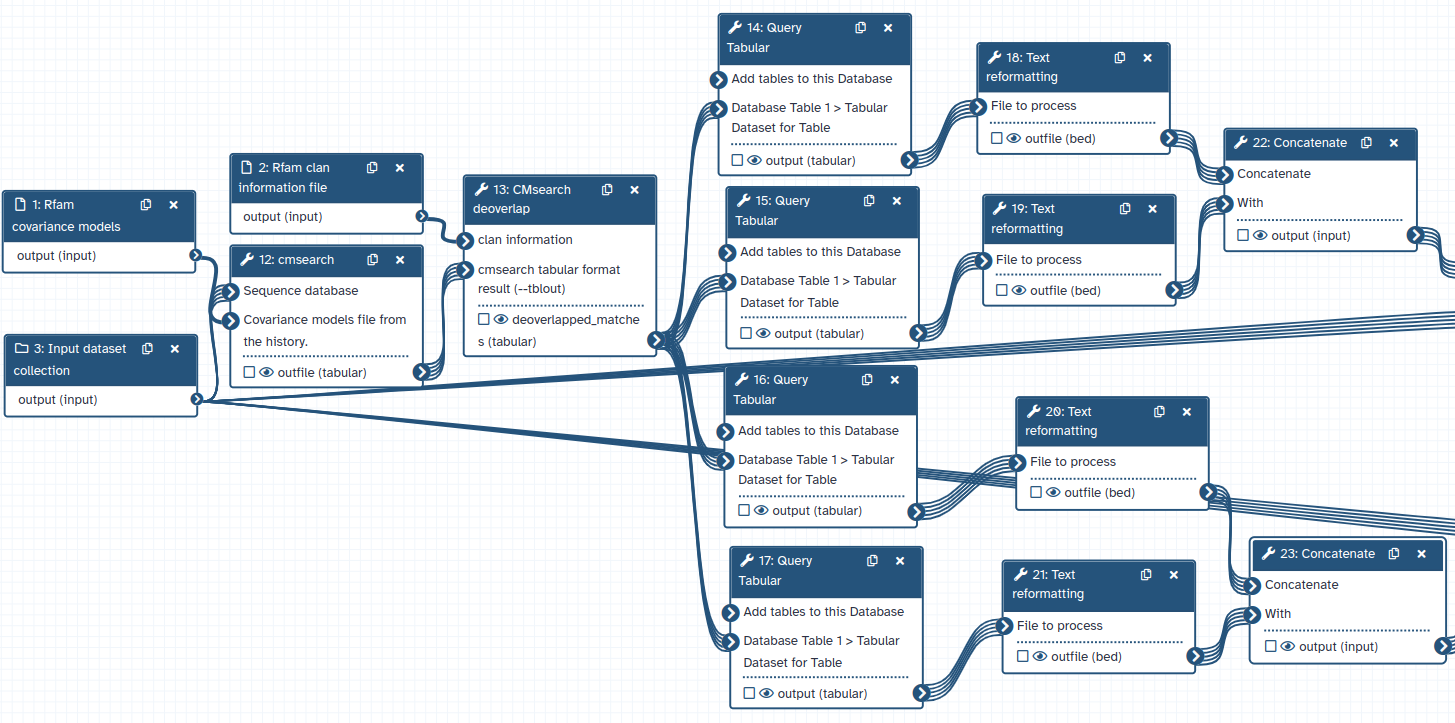
\includegraphics[width=\paperwidth,height=\paperheight,keepaspectratio]{figures/Galaxy_WF_part1.png}
  \captionof{figure}[Galaxy-ported version of rRNA-prediction subworkflow (part 1)]{\textbf{Galaxy-ported version of rRNA-prediction subworkflow (Part 1)}. The initial part of the rRNA-prediction subworkflow within the Galaxy interface. The link to the Galaxy-ported rRNA-prediction subworkflow can be found in \Cref{appendix_galaxy_workflows}} \label{fig:Galaxy_WF_part1}%
\end{center}

\end{landscape}
\begin{figure}[H]
  \centering
  \subfloat{{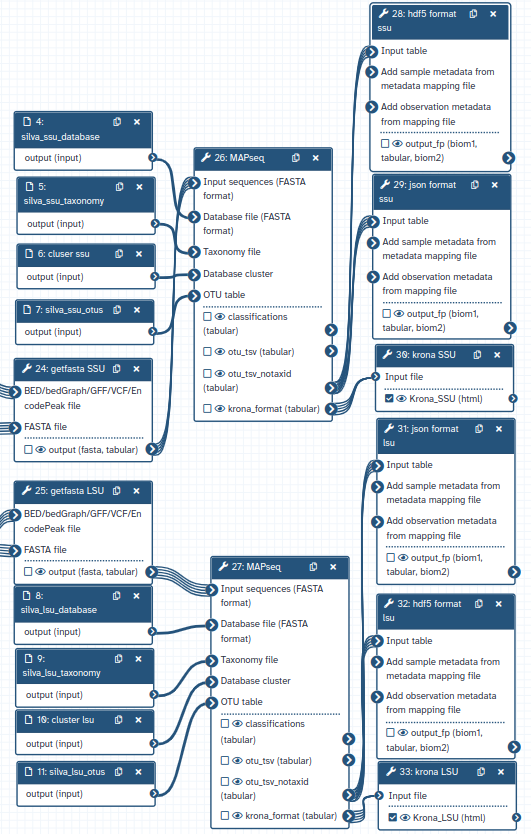
\includegraphics[scale=0.6]{figures/Galaxy_WF_part2.png} }}%
  \captionof{figure}[Galaxy-ported version of rRNA-prediction subworkflow (part 2)]{\textbf{Galaxy-ported version of rRNA-prediction subworkflow (Part 2)}. The second part of the rRNA-prediction subworkflow within the Galaxy interface. Where getfasta SSU and getfasta LSU receive the SSU and LSU BED files from Concatenate (Tool IDs 22 and 23 in \Cref{fig:Galaxy_WF_part1})} \label{fig:Galaxy_WF_part2}%
\end{figure}
\begin{figure}[H]
  \centering
  \subfloat{{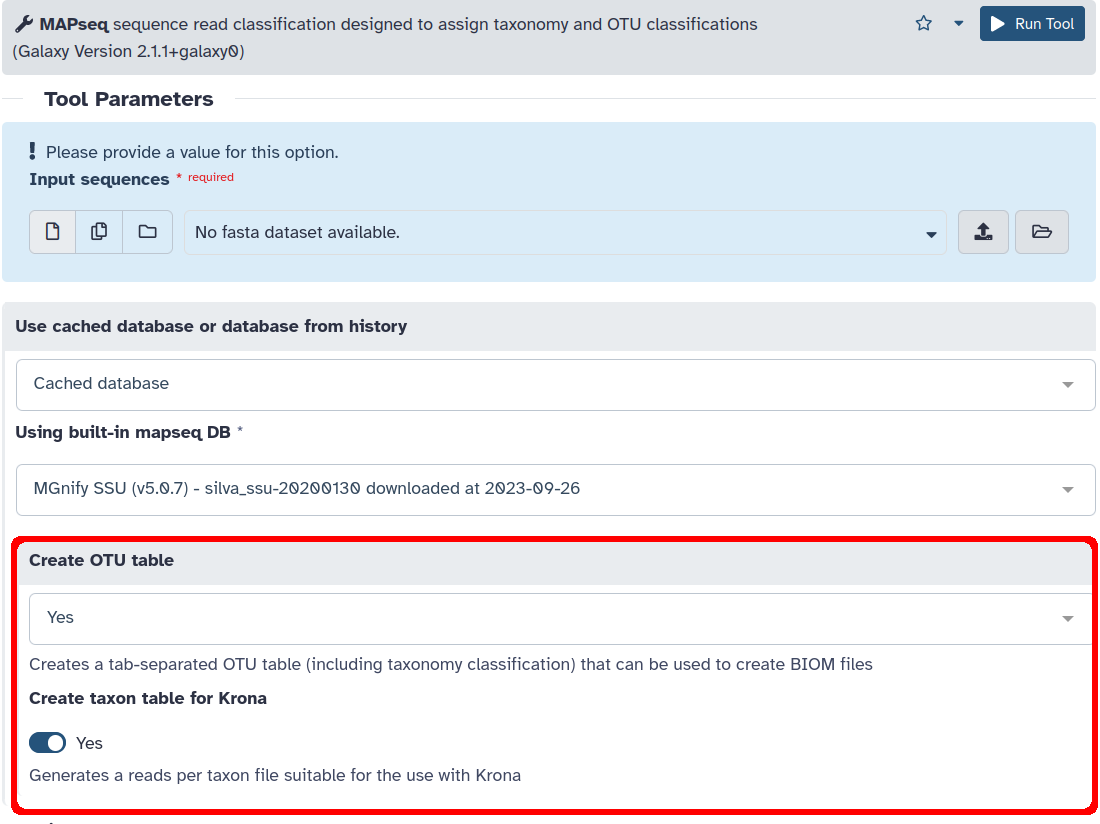
\includegraphics[scale=0.36]{figures/MAPseq.png} }}%
  \captionof{figure}[MAPseq tool in Galaxy]{\textbf{GUI view of the MAPseq tool in Galaxy}~\cite{noauthor_tools-iuctoolsmapseq_nodate}. including the mapseq2biom tool as an option (outlined in red).} \label{fig:MAPseq}%
\end{figure}